\documentclass[a4paper,USenglish,cleveref,autoref]{lipics-v2021}
\hideLIPIcs
\usepackage{amsmath,amssymb,tikz}
\usetikzlibrary{arrows.meta}
\bibliographystyle{plainurl}
\title{Primitive Words Have No Finitely Ambiguous Context-Free Grammar}
\titlerunning{Primitive Words Have No Finitely Ambiguous Grammar}
\author{Author name to be supplied}{Affiliation and country to be supplied}{}{}{}
\authorrunning{Author metadata pending}
\Copyright{Author name to be supplied}
\ccsdesc[500]{Theory of computation~Grammars and context-free languages}
\keywords{Primitive words, context-free grammars, bounded ambiguity, bounded languages, stratified semilinear sets}
\category{Research manuscript draft}
\newcommand{\N}{\mathbb N}
\newcommand{\Z}{\mathbb Z}
\newcommand{\R}{\mathbb R}
\newcommand{\Q}{\mathcal Q}
\newcommand{\NE}{\mathrm{NE}}
\newcommand{\spanR}{\operatorname{span}_{\R}}
\newcommand{\cone}{\operatorname{cone}}
\newcommand{\supp}{\operatorname{supp}}
\newcommand{\amb}{\operatorname{amb}}
\newcommand{\rank}{\operatorname{rank}}
\begin{document}
\maketitle
\begin{abstract}
A nonempty word is primitive if it is not a proper power.
Petersen proved that the language of primitive words over an alphabet with at least two letters is not unambiguous context-free.
We show that it admits no context-free grammar with a uniform finite bound on the number of derivation trees of a word.
More precisely, for $M\geq 1$, every context-free grammar generating the primitive words in the regular language $a(ab^+)^M a(ab^+)^M$ has a word with at least $\lceil(M+1)/2\rceil$ derivation trees.
The proof uses the classical characterization of bounded finite-ambiguity languages by covers with stratified simple linear sets.
A noncrossing rank lemma shows that, near a generic point of the diagonal and on a suitable sublattice, each relevant linear set becomes a strict half-space in the transverse coordinates.
A covering argument then forces increasing overlap.
The result does not decide whether the language of primitive words is context-free.
\end{abstract}

\section{Introduction}
A word is \emph{primitive} if it cannot be written as $u^r$ with $r\geq 2$.
Let $\Q_A$ denote the language of nonempty primitive words over a finite alphabet $A$.
The context-freeness of $\Q_A$, for $|A|\geq 2$, is a longstanding open problem in formal-language theory; surveys and recent work continue to distinguish this question from the known impossibility of unambiguous generation~\cite{Lischke2011,Amarilli2026}.
The distinction matters because ambiguity concerns the number of descriptions of a word, rather than membership alone.

Petersen proved that $\Q_A$ is not an unambiguous context-free language~\cite{Petersen1994,Petersen1996}.
The 1996 article is the journal version of the 1994 conference paper.
Koechlin subsequently gave another proof using a bounded intersection and generating functions~\cite[Proposition 17]{Koechlin2022}.
These results rule out one derivation tree per word, but do not by themselves rule out a fixed bound of two, three, or any other finite number of trees.

We exclude every such bound.
Throughout, \emph{finitely ambiguous} means that one constant bounds the number of derivation trees of \emph{every} word.
It does not mean merely that each word has finitely many trees.

\begin{theorem}\label{thm:main}
Let $A$ be a finite alphabet with at least two letters.
For every context-free grammar $G$ with $L(G)=\Q_A$ and every $k\in\N$, there is a word $w\in\Q_A$ with more than $k$ derivation trees in $G$.
\end{theorem}

Our argument gives a quantitative obstruction on regular slices.
Fix distinct letters $a,b$ and write $\Q=\Q_{\{a,b\}}$.
For $M\geq 1$, set
\begin{equation}\label{eq:slice}
 R_M=a(ab^+)^M a(ab^+)^M,\qquad L_M=\Q\cap R_M.
\end{equation}
\begin{theorem}\label{thm:slice}
Every context-free grammar generating $L_M$ has a word with at least $\lceil(M+1)/2\rceil$ derivation trees.
\end{theorem}
The number of occurrences of $a$ in this slice is $2M+2$.
Thus, an assumed ambiguity bound $k\geq1$ is contradicted by the single slice with $M=2k$.
The lower bound is not asserted to be the exact ambiguity degree of every slice.

\paragraph{Proof idea.}
The two initial adjacent occurrences of $a$ mark the starts of two halves of a slice word.
A proper power in $R_M$ must be a square, so the primitive words correspond exactly to pairs of distinct positive integer vectors $(x,y)$.
The classical bounded-language characterization translates a grammar with ambiguity at most $k$ into a finite cover of these vectors by simple stratified linear sets, with overlap at most $k$~\cite{GinsburgUllian1966,Rosenberg1970,Koechlin2022}.
Stratification requires periods to involve at most two coordinates, with noncrossing supports.
The coordinate pairs expressing $x_i=y_i$ cross pairwise in the order $x_1,\ldots,x_M,y_1,\ldots,y_M$.

The central step exploits this conflict.
If noncrossing nonnegative periods span the diagonal subspace, their rank is at least $2M-1$.
Consequently, near a generic positive diagonal direction, a simple linear set that avoids the diagonal has at most one active transverse inequality.
Passing to a common sublattice removes congruence obstructions, and the surviving sets become strict half-spaces through the origin in $\R^M$.
Covering all nonzero directions requires at least $M+1$ such half-spaces.
At a pair of opposite generic directions, their overlap counts sum to the number of half-spaces, proving the bound.

\paragraph{Relation to earlier work.}
The structural characterization of finitely ambiguous bounded languages is classical; we use the formulation recalled by Koechlin~\cite[p.~41:16]{Koechlin2022}, with explicit care about the exponent encoding.
Koechlin proves non-unambiguity of primitive words using a three-block slice and discusses higher ambiguity degrees as a direction for further work.
Our argument instead uses a family of slices of increasing dimension and a geometric overlap lower bound.
The mathematical contribution presented here is this quantitative obstruction, rather than a new semilinear characterization.
If $\Q_A$ is context-free, the main theorem implies that every grammar for it has unbounded ambiguity; it supplies neither a grammar for $\Q_A$ nor a proof of non-context-freeness.

\section{Preliminaries and the bounded-language interface}
We use $\N=\{0,1,2,\ldots\}$ and write $\N_{>0}$ for the positive integers.
Derivation trees are finite ordered trees labeled by grammar rules; distinct copies of an identical production are not different rules.
For a context-free grammar $G$, let $\amb_G(w)\in\N\cup\{\infty\}$ be the number of its derivation trees with yield $w$.
A grammar is \emph{$k$-ambiguous} if $\amb_G(w)\leq k$ for every word $w$.

A \emph{linear set} in $\N^d$ has the form
\begin{equation}\label{eq:linear}
 L=c+\N v_1+\cdots+\N v_r,
 \qquad c\in\N^d,\quad v_j\in\N^d\setminus\{0\}.
\end{equation}
It is \emph{simple} if its periods $v_1,\ldots,v_r$ are linearly independent over $\R$.
The support of a vector is the set of its nonzero coordinates.
A period family is \emph{stratified} if each support has size at most two, and there do not exist two supports $\{i,k\}$ and $\{j,\ell\}$ with $i<j<k<\ell$.
Singleton supports and shared endpoints are permitted.
We also call this support condition \emph{noncrossing}.

For a finite indexed family $(L_\alpha)_{\alpha\in I}$, its multiplicity at $z$ is
\begin{equation}\label{eq:ply}
 f(z)=\sum_{\alpha\in I}\mathbf 1_{L_\alpha}(z).
\end{equation}
Indices are counted separately, even if two members are equal.
A cover has multiplicity at most $k$ if $f(z)\leq k$ everywhere.

We use the following classical implication for letter-bounded languages.
It is the finite-ambiguity characterization of Ginsburg--Ullian and Rosenberg, in the form recalled in the conclusion of Koechlin~\cite{GinsburgUllian1966,Rosenberg1970,Koechlin2022}.
\begin{theorem}[Classical bounded-language implication]\label{thm:classical}
Let $c_1,\ldots,c_d$ be distinct letters and let $K\subseteq c_1^*\cdots c_d^*$ admit a $k$-ambiguous context-free grammar.
Then its exponent set
\[
 E(K)=\{(n_1,\ldots,n_d):c_1^{n_1}\cdots c_d^{n_d}\in K\}
\]
is a finite union of simple stratified linear sets with multiplicity at most $k$.
\end{theorem}
The independence and overlap conclusions are essential.
Ordinary semilinearity alone does not provide either of them.

\begin{lemma}[Unique positional lift]\label{lem:lift}
Suppose $L\subseteq (ab^*)^n$ admits a $k$-ambiguous context-free grammar.
Then
\[
 E_n(L)=\{(z_1,\ldots,z_n):ab^{z_1}\cdots ab^{z_n}\in L\}
\]
is a finite union of simple stratified linear sets with multiplicity at most $k$.
\end{lemma}
\begin{proof}
Introduce distinct letters $A_1,B_1,\ldots,A_n,B_n$ and the letter homomorphism $h$ given by $h(A_i)=a$ and $h(B_i)=b$.
Put
\[
 T=A_1B_1^*\cdots A_nB_n^*,\qquad \widetilde L=h^{-1}(L)\cap T.
\]
Every word $ab^{z_1}\cdots ab^{z_n}$ has exactly one preimage in $T$, namely $A_1B_1^{z_1}\cdots A_nB_n^{z_n}$.
Moreover, for any fixed lifted word, replacing each terminal occurrence in an original derivation tree by the corresponding lifted letter is unique.
A grammar for $h^{-1}(L)$ can be obtained by allowing all inverse letter choices at terminal occurrences in each rule.
For a fixed lifted yield, its trees correspond bijectively to the original trees for its image under $h$.
Intersection with the deterministic automaton for $T$ preserves this count: each subtree has uniquely determined entry and exit states in the accepting run.
Thus $\widetilde L$ has a $k$-ambiguous grammar.

Apply Theorem~\ref{thm:classical} in the order $A_1,B_1,\ldots,A_n,B_n$.
Every resulting linear set lies in the exponent set of $\widetilde L$, where all $A_i$ coordinates equal one.
Its periods therefore vanish on those coordinates.
Deleting them preserves independence, supports, and their noncrossing order.
It also preserves cover multiplicity, because the deleted coordinates are fixed.
The resulting family covers exactly $E_n(L)$.
\end{proof}

For completeness, these tree-count observations do not assume that the input grammar is unambiguous or in a particular normal form.
For a general production, state annotations may be put at every position on its right-hand side; the deterministic run fixes them uniquely on a completed tree.
For the empty word, the same entry and exit state are used.

\section{A regular slice of primitive words}
Every word of $R_M$ has a unique expression
\begin{equation}\label{eq:word}
 w(x,y)=a\prod_{i=1}^M(ab^{x_i})\;a\prod_{i=1}^M(ab^{y_i}),
 \qquad x,y\in\N_{>0}^M.
\end{equation}
The corresponding block exponent vector in $(ab^*)^{2M+2}$ is $(0,x_1,\ldots,x_M,0,y_1,\ldots,y_M)$.
The positive-exponent condition makes the two zero coordinates distinguishable markers.

\begin{lemma}\label{lem:slice}
The word $w(x,y)$ is primitive if and only if $x\ne y$.
\end{lemma}
\begin{proof}
If $x=y$, the two displayed halves agree, so $w(x,y)$ is a square.
Conversely, suppose $w(x,y)=u^r$ with $r\geq2$.
The word $u$ begins with $a$, since $w(x,y)$ does.
Each copy of $u$ therefore begins at an $a$-boundary, and $u$ contains exactly $s=(2M+2)/r$ occurrences of $a$.
The cyclic block exponent vector is invariant under a shift by $s$, where $0<s<2M+2$.
This shift must preserve its zero set $\{1,M+2\}$.
It cannot fix position $1$, so it sends $1$ to $M+2$, giving $s=M+1$ and $r=2$.
Invariance under this shift says precisely $x=y$.
\end{proof}

Define the diagonal subspace and the positive off-diagonal integer set by
\begin{equation}\label{eq:diagonal}
 W=\{(u,u):u\in\R^M\},\qquad
 \NE_M=\{(x,y)\in\N_{>0}^{2M}:x\ne y\}.
\end{equation}
If $L_M$ has a $k$-ambiguous grammar, Lemma~\ref{lem:lift} gives a cover of its block exponent set by simple stratified linear sets of multiplicity at most $k$.
The two zero marker coordinates are zero in every base and period.
Deleting them preserves all structural conditions and gives a cover of $\NE_M$ with multiplicity at most $k$.
Every member of this cover is disjoint from $W$.

\section{Noncrossing supports force almost full rank}
We next isolate the linear-algebraic obstruction.
All coordinates are ordered as $x_1,\ldots,x_M,y_1,\ldots,y_M$.
In this order, two distinct matched pairs $\{i,M+i\}$ and $\{j,M+j\}$ cross, as illustrated in Figure~\ref{fig:geometry}.

\begin{figure}[t]
\centering
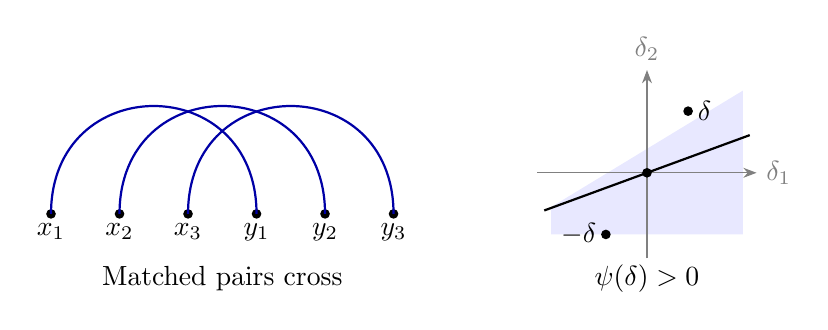
\begin{tikzpicture}[>=Stealth,scale=.87]
\foreach \i/\s in {0/$x_1$,1/$x_2$,2/$x_3$,3/$y_1$,4/$y_2$,5/$y_3$}{\fill (\i,0) circle (2pt);\node[below] at (\i,0){\s};}
\draw[thick,blue!65!black] (0,0) .. controls (0,2.1) and (3,2.1) .. (3,0);
\draw[thick,blue!65!black] (1,0) .. controls (1,2.1) and (4,2.1) .. (4,0);
\draw[thick,blue!65!black] (2,0) .. controls (2,2.1) and (5,2.1) .. (5,0);
\node at (2.5,-.95) {Matched pairs cross};
\begin{scope}[xshift=8.7cm,yshift=.6cm]
\fill[blue!9] (-1.4,-.9)--(1.4,-.9)--(1.4,1.2)--(-1.4,-.5)--cycle;
\draw[gray,->] (-1.6,0)--(1.6,0) node[right] {$\delta_1$};
\draw[gray,->] (0,-1.25)--(0,1.5) node[above] {$\delta_2$};
\draw[thick] (-1.5,-.55)--(1.5,.55);
\fill (0,0) circle (2pt);
\fill (.6,.9) circle (2pt) node[right] {$\delta$};
\fill (-.6,-.9) circle (2pt) node[left] {$-\delta$};
\node at (0,-1.55) {$\psi(\delta)>0$};
\end{scope}
\end{tikzpicture}
\caption{The diagonal imposes crossing matched pairs (left, $M=3$), whereas periods in each stratified set have noncrossing supports.
After lattice scaling, each surviving set contributes a strict half-space in transverse coordinates (right, $M=2$).
Exactly one of two generic opposite directions belongs to each such half-space.}
\label{fig:geometry}
\end{figure}

\begin{lemma}[Components do not interleave]\label{lem:components}
Let a graph have linearly ordered vertices and pairwise noncrossing edges.
Two different connected components cannot contain vertices $p<q<r<s$ with $p,r$ in one component and $q,s$ in the other.
\end{lemma}
\begin{proof}
Suppose components $C,D$ have such vertices.
A path in $C$ from $p$ to $r$ has an edge $\{a,b\}$ with $a<q<b$.
No edge of $D$ can leave $(a,b)$: its endpoints cannot equal $a,b$, and such an edge would cross $\{a,b\}$.
Connectivity implies $D\subseteq(a,b)$.
Likewise, a path in $D$ from $q$ to $s$ has an edge $\{c,d\}$ with $c<r<d$, and then $C\subseteq(c,d)$.
But $c,d\in(a,b)$, so $a\notin(c,d)$, contradicting $a\in C$.
\end{proof}

\begin{lemma}[Noncrossing rank bound]\label{lem:rank}
Let $V$ be a finite family of nonzero nonnegative vectors in $\R^{2M}$ whose supports have size at most two and are noncrossing.
If $W\subseteq\spanR V$, then
\begin{equation}\label{eq:rank}
 \dim\spanR V\geq 2M-1.
\end{equation}
\end{lemma}
\begin{proof}
Form the support graph on $\{1,\ldots,2M\}$, with an edge for each two-element support and a loop for each singleton support.
For a connected component $C$, let $V_C$ consist of its vectors and put $U_C=\spanR V_C\subseteq\R^C$.
Since different components have disjoint supports,
\[
 \spanR V=\bigoplus_C U_C.
\]
The vectors on the edges of a spanning tree of $C$ are independent: remove a leaf and use its positive coordinate to eliminate its incident edge coefficient, then repeat.
Consequently $\dim U_C\geq |C|-1$.
Call $C$ deficient if $U_C\ne\R^C$.

For a deficient component, $U_C$ is the kernel of a nonzero linear form $\lambda$ on $\R^C$.
An edge vector $\alpha e_p+\beta e_q$, with $\alpha,\beta>0$, implies $\alpha\lambda_p+\beta\lambda_q=0$.
Thus a zero coordinate of $\lambda$ propagates along edges, and connectivity shows that $\lambda$ vanishes nowhere.
This also covers an isolated vertex directly.
In particular, $e_p\notin U_C$ for every $p\in C$.

The vector $e_i+e_{M+i}$ belongs to $\spanR V$.
If $i$ and $M+i$ were in different components, projection onto either component would show that its corresponding coordinate vector lies in $U_C$.
It follows that every deficient component is a union of matched pairs $\{i,M+i\}$.
Two deficient components would therefore contain different matched pairs, which interleave.
Lemma~\ref{lem:components} excludes this possibility.
At most one component is deficient, and summing the component ranks gives~\eqref{eq:rank}.
\end{proof}

\section{From linear sets to transverse half-spaces}
We prove the covering bound needed for the slice theorem.
This part of the argument separates the real cone geometry from the arithmetic of the period lattices; both are necessary.

\begin{theorem}[Cover multiplicity bound]\label{thm:cover}
Let $(L_\alpha)_{\alpha\in I}$ be a finite cover of $\NE_M$ by simple stratified linear sets, each contained in $\NE_M$.
Then some point of $\NE_M$ lies in at least $\lceil(M+1)/2\rceil$ members of the cover.
\end{theorem}
\begin{proof}
Write $L_\alpha=c_\alpha+\N V_\alpha$ and $U_\alpha=\spanR V_\alpha$.
For each index, consider the rational polyhedral cone
\begin{equation}\label{eq:C}
 C_\alpha=\{u\in\R^M:(u,u)\in\cone(V_\alpha)\}.
\end{equation}
Choose $\omega\in\Z_{>0}^M$ outside the boundaries of all these cones.
Such a choice exists because each boundary is contained in finitely many proper linear subspaces; a lower-dimensional cone is its own boundary.
Thus either $\omega\notin C_\alpha$ or $\omega\in\operatorname{int}C_\alpha$ for every $\alpha$.

\paragraph{Periods positive in the diagonal direction.}
Suppose $\omega\in\operatorname{int}C_\alpha$.
Then $W\subseteq U_\alpha$.
Since $V_\alpha$ is independent, each $v\in V_\alpha$ has a coefficient functional $n_v:U_\alpha\to\R$ characterized by $z=\sum_v n_v(z)v$.
These functionals are nonnegative on the period cone.
Define
\[
 V_\alpha^+=\{v:n_v|_W\ne0\},\qquad
 V_\alpha^0=\{v:n_v|_W=0\}.
\]
For $v\in V_\alpha^+$, we have $n_v(\omega,\omega)>0$.
Indeed, a linear form nonnegative on a neighborhood of $\omega$ that vanishes at $\omega$ must vanish identically.
Moreover, $W\subseteq\spanR V_\alpha^+$, by expansion in the basis $V_\alpha$.
The rank bound therefore gives
\begin{equation}\label{eq:positive}
 |V_\alpha^+|\geq2M-1,\qquad |V_\alpha^0|\leq1.
\end{equation}
In particular, $\dim U_\alpha$ is either $2M-1$ or $2M$.

\paragraph{A common arithmetic scale.}
For every index, let
\[
 \Lambda_\alpha=U_\alpha\cap\Z^{2M},\qquad
 I_\alpha=[\Lambda_\alpha:\Z V_\alpha].
\]
The index is finite, with value one in rank zero.
For each interior-cone index of rank $2M-1$, choose a nonzero integral form $\lambda_\alpha$ with $U_\alpha=\ker\lambda_\alpha$.
For each full-rank interior-cone index with $V_\alpha^0=\{v_*\}$, put
\[
 \gamma_\alpha=n_{v_*}(c_\alpha),\qquad
 D_\alpha=|\det V_\alpha|.
\]
Choose one positive integer $F$ divisible by every $I_\alpha$ and sufficiently large that
\begin{equation}\label{eq:F}
 F>|\lambda_\alpha(c_\alpha)|,
 \qquad F>D_\alpha\max\{\gamma_\alpha,0\}
\end{equation}
whenever the respective quantities are defined.
These are finitely many conditions depending only on the cover and $\omega$.

We will use the following lattice observation.
If $L_\alpha$ contains a point $z_1\in F\Z^{2M}$, then every
$z\in F\Z^{2M}\cap(c_\alpha+U_\alpha)$ satisfies
\begin{equation}\label{eq:lattice}
 z-c_\alpha\in\Z V_\alpha.
\end{equation}
Indeed, $z-z_1\in F\Lambda_\alpha\subseteq\Z V_\alpha$, since $I_\alpha\Lambda_\alpha\subseteq\Z V_\alpha$.
Adding $z_1-c_\alpha\in\N V_\alpha$ proves the observation.

\paragraph{Classification near the diagonal.}
For $\delta\in\Z^M$ and $t\in F\Z_{>0}$, set
\begin{equation}\label{eq:P}
 P(t,\delta)=(t\omega,t\omega+F\delta).
\end{equation}
Fix any finite perturbation window $\|\delta\|_\infty\leq R$.
We classify membership for all sufficiently large $t$; the threshold may depend on $R$, but $\omega$ and $F$ do not.

If $\omega\notin C_\alpha$, then $P(t,\delta)\notin L_\alpha$ eventually throughout this window.
Otherwise, a fixed $\delta$ would occur for unboundedly many $t$, and division of $P(t,\delta)-c_\alpha\in\cone(V_\alpha)$ by $t$, followed by closedness of the cone, would give $(\omega,\omega)\in\cone(V_\alpha)$.
This contradicts the choice of the case.

Now suppose $\omega\in\operatorname{int}C_\alpha$ and $\dim U_\alpha=2M-1$.
By~\eqref{eq:positive}, all its coefficient functionals are positive at $(\omega,\omega)$.
If $L_\alpha$ contained any $P(t,\delta)$, then
\[
 \lambda_\alpha(c_\alpha)
 =\lambda_\alpha(P(t,\delta))
 =F\lambda_\alpha(0,\delta)\in F\Z,
\]
because $\lambda_\alpha$ vanishes on $W$.
Condition~\eqref{eq:F} forces $\lambda_\alpha(c_\alpha)=0$.
Hence $c_\alpha\in U_\alpha$, and every diagonal point $P(s,0)$ lies in the affine span $c_\alpha+U_\alpha$.
For large $s\in F\Z_{>0}$, the lattice observation gives integer coefficients for $P(s,0)-c_\alpha$.
All are positive for sufficiently large $s$, since they equal
$s n_v(\omega,\omega)-n_v(c_\alpha)$.
This puts a diagonal point in $L_\alpha$, a contradiction.
Such an index therefore contributes no sample point.

If the rank is $2M$ and $V_\alpha^0$ is empty, the same argument applies without $\lambda_\alpha$.
One sample point gives the lattice condition for every diagonal sample point, and all coefficients eventually become nonnegative.
This case also contributes no sample point.

The only remaining case has rank $2M$ and $V_\alpha^0=\{v_*\}$.
Discard such an index if it contains no sample point at all.
For every remaining index define the nonzero rational linear form
\begin{equation}\label{eq:psi}
 \psi_\alpha(\delta)=n_{v_*}(0,\delta).
\end{equation}
It is nonzero because $n_{v_*}$ is nonzero and vanishes on $W$, while $\R^{2M}=W\oplus(\{0\}\times\R^M)$.
The lattice observation supplies integer coefficients for every sample point minus the base.
All coefficients other than the $v_*$ coefficient eventually become positive, uniformly in the finite window.
The remaining coefficient is $F\psi_\alpha(\delta)-\gamma_\alpha$.
Therefore
\begin{equation}\label{eq:threshold}
 P(t,\delta)\in L_\alpha
 \quad\Longleftrightarrow\quad
 F\psi_\alpha(\delta)\geq\gamma_\alpha
 \qquad(t\text{ sufficiently large}).
\end{equation}
Necessarily $\gamma_\alpha>0$, since otherwise $\delta=0$ in~\eqref{eq:threshold} gives a forbidden diagonal point.
Cramer's rule gives $\psi_\alpha(\Z^M)\subseteq D_\alpha^{-1}\Z$.
Together with~\eqref{eq:F}, this turns~\eqref{eq:threshold} into
\begin{equation}\label{eq:halfspace}
 P(t,\delta)\in L_\alpha
 \quad\Longleftrightarrow\quad \psi_\alpha(\delta)>0.
\end{equation}

\paragraph{Counting half-spaces.}
Let $H$ be the indexed family of remaining indices in the last case.
Its definition uses the existence of any sample point, so it is independent of $R$.
Taking a common threshold over the finite cover, and increasing it beyond $FR$, yields for every nonzero integral $\delta$ in the window
\begin{equation}\label{eq:eventual}
 1\leq f(P(t,\delta))
 =\#\{\alpha\in H:\psi_\alpha(\delta)>0\}.
\end{equation}
Here positivity of the coordinates follows from $t>FR$ and $\omega_i\geq1$; the point is off the diagonal because $\delta\ne0$.
Since the window was arbitrary, the half-spaces cover all nonzero integral vectors.

The rational polyhedral cone
\[
 K=\bigcap_{\alpha\in H}\{\delta\in\R^M:\psi_\alpha(\delta)\leq0\}
\]
contains no nonzero integral point.
A nonzero rational polyhedral cone has a nonzero rational point, and hence a nonzero integral point after scaling.
Thus $K=\{0\}$.
The forms must span the dual of $\R^M$, since otherwise their common kernel is nonzero.
There must in fact be at least $M+1$ forms: if there were exactly $M$, spanning would make them independent, and the system $\psi_\alpha(\delta)=-1$ would have a solution in $K\setminus\{0\}$.

Choose $\delta\in\Z^M$ outside all the kernels of these finitely many nonzero rational forms.
For each index, exactly one of $\psi_\alpha(\delta)$ and $\psi_\alpha(-\delta)$ is positive.
Choose a window containing both directions and then one sufficiently large $t$ for~\eqref{eq:eventual}.
It follows that
\[
 f(P(t,\delta))+f(P(t,-\delta))=|H|\geq M+1.
\]
At least one of these two off-diagonal points has multiplicity at least $\lceil(M+1)/2\rceil$, as required.
\end{proof}

\section{Consequences for grammars of primitive words}
The preceding theorem concerns arbitrary covers with the stated geometry.
The grammar-theoretic conclusions now follow from the positional lift and deterministic regular intersection.

\begin{proof}[Proof of Theorem~\ref{thm:slice}]
Put $q=\lceil(M+1)/2\rceil$.
If $q=1$, the conclusion holds because $L_M$ is nonempty: choose positive $x\ne y$ and apply Lemma~\ref{lem:slice}.
If a grammar for $L_M$ had fewer than $q$ trees for every word, it would be $(q-1)$-ambiguous.
The construction after Lemma~\ref{lem:slice} would give a simple stratified cover of $\NE_M$ of multiplicity at most $q-1$.
This contradicts Theorem~\ref{thm:cover}.
\end{proof}

\begin{proof}[Proof of Theorem~\ref{thm:main}]
First consider the binary alphabet.
Suppose a grammar $G$ for $\Q$ is $k$-ambiguous.
As $a\in\Q$, necessarily $k\geq1$.
Intersect $G$ with a deterministic automaton for $R_{2k}$.
Each accepted derivation tree has a unique state annotation, so the resulting grammar generates $L_{2k}$ with ambiguity at most $k$.
Theorem~\ref{thm:slice} supplies a word with at least $\lceil(2k+1)/2\rceil=k+1$ trees, a contradiction.

For a finite alphabet $A$ containing $a,b$, intersect a proposed $k$-ambiguous grammar for $\Q_A$ with $\{a,b\}^*$.
Primitivity of a word using only $a,b$ is unchanged when it is viewed over $A$: any root of that word also uses only its letters.
Thus the intersection is exactly $\Q$, and deterministic intersection again preserves the bound.
The binary case gives the contradiction.
\end{proof}

The argument does not require a cycle-free hypothesis on the grammar.
If a useful derivation cycle produces infinitely many trees for a word, the conclusion already holds; otherwise the bounded-language implication applies under the hypothesized uniform finite bound.
No inference about the context-freeness of the full primitive-word language is used.

\section{Proof artifacts and further questions}
The accompanying repository contains the written proof, separate structural and geometric audit reports, finite computational checks, and a Lean development~\cite{Artifact}.
The formalization states the binary theorem for cycle-free context-free grammars, using an explicit definition of uniform finite ambiguity.
It develops a direct grammar-to-cover argument rather than importing the classical bounded-language characterization used here.
The source includes the regular slice, normal-form conversion, structural representation, noncrossing rank argument, and geometric obstruction.

The repository reports a build with Lean 4.36.0 and Mathlib v4.36.0 and an axiom report containing only \texttt{propext}, \texttt{Classical.choice}, and \texttt{Quot.sound}.
The preparation of this draft inspected the definitions and source but did not independently rerun that pinned build, because the required toolchain was unavailable in the drafting environment.
The extension to larger alphabets and the unrestricted grammar statement are justified by the written reductions above; they are not claimed as the exact statement of the archived Lean theorem.
Computational searches are supporting checks, not premises of the proof.

The lower bound leaves two natural questions.
One is the exact ambiguity degree of each $L_M$; the present argument proves a growing lower bound but does not establish its sharpness.
The other is whether the geometric obstruction can be extended beyond uniformly bounded ambiguity.
Resolving that question would require additional information about arbitrary context-free grammars, because the finite-cover multiplicity interface is precisely where the uniform bound enters.

\section*{Use of generative AI}
The author reports using Claude Opus 5.5 in medium mode during the mathematical discovery process.
The work proceeded through guided, iterative interaction: an initial request to resolve the whole conjecture did not succeed, and the author subsequently decomposed the problem and indicated prior results on which to build.
AI assistance contributed to mathematical exploration and proof development; the retained repository also contains AI-assisted proof audits, computational checks, and Lean formalization work.
Codex assisted with the literature review, mathematical exposition, bibliography preparation, and typesetting of this manuscript draft.

Complete original conversation transcripts and exact discovery prompts were not retained in the repository.
The available reports and proof sources document part of the development, but later prompts concerning the remaining context-freeness problem are not the original discovery prompts.
The present statement records the reported human guidance and the available artifacts; it does not claim autonomous discovery or a completed independent human verification of every argument.
The scope of the final author review and approval remains to be confirmed before submission.

\bibliography{references}
\end{document}
